\documentclass[10pt]{article}
\usepackage[margin=0.8in]{geometry}
\usepackage[utf8]{inputenc}
\usepackage[T1]{fontenc}
\usepackage[english]{babel}

\usepackage{fourier}
\usepackage{amsmath}
\usepackage{amssymb}
\usepackage{amsfonts}
\usepackage{amsthm}

\usepackage{graphicx}
\usepackage{float}
\usepackage{caption}
\usepackage{subcaption}

\usepackage{booktabs}

\usepackage{etoolbox}
\usepackage{siunitx}
\usepackage{parskip} % Creates space between paragraphs instead of indentation
\setlength{\parskip}{1em} % Adjust space between paragraphs
\setlength{\parindent}{0pt} % No indentation

\usepackage{hyperref}
\hypersetup{
    colorlinks=true,
    linkcolor=blue,
    filecolor=magenta,
    urlcolor=cyan,
}
\usepackage{cite}

\usepackage{listings}
\usepackage{color}

\definecolor{codegreen}{rgb}{0,0.6,0}
\definecolor{codegray}{rgb}{0.5,0.5,0.5}
\definecolor{codepurple}{rgb}{0.58,0,0.82}
\definecolor{backcolour}{rgb}{0.95,0.95,0.92}

\lstdefinestyle{mystyle}{
    backgroundcolor=\color{backcolour},
    commentstyle=\color{codegreen},
    keywordstyle=\color{magenta},
    numberstyle=\tiny\color{codegray},
    stringstyle=\color{codepurple},
    basicstyle=\ttfamily\footnotesize,
    breakatwhitespace=false,
    breaklines=true,
    captionpos=b,
    keepspaces=true,
    numbers=left,
    numbersep=5pt,
    showspaces=false,
    showstringspaces=false,
    showtabs=false,
    tabsize=2,
    language=C++
}
\lstset{style=mystyle}

\newcommand{\code}[1]{\texttt{#1}}


\title{Assignment 3: Miniz-based parallel compressor/decompressor in OpenMP}
\author{Luca Lombardo \\ SPM Course a.a. 24/25}
\date{May 2, 2025}

\begin{document}

\maketitle
\vspace{-1.5em} % Reduce space after title block

\section{Parallelization Strategies}

To compress files efficiently in parallel with OpenMP, we needed different strategies for different kinds of input. Our implementation handles three main cases. When dealing with many small files, we use task parallelism. Each file is an independent task assigned to threads using an OpenMP \code{parallel for} loop. Since file sizes can vary quite a bit, we use \code{dynamic} scheduling for better load balancing. If a file is smaller than a set threshold (default 16 MiB), the assigned thread processes it sequentially; this avoids the overhead of parallelizing tiny tasks where blocks wouldn't help much.

For a single large file larger than the threshold, we switch to data parallelism. We split the file into fixed-size blocks (default 1 MiB, but adjustable). An OpenMP \code{parallel for} loop then lets threads work on these blocks together. To keep things thread-safe, each thread gets its own Miniz compressor instance. Choosing the block size here is a trade-off: smaller blocks allow for more granular work distribution but add overhead for managing block metadata and might slightly hurt compression because each block has less context. Larger blocks reduce this overhead but risk uneven workloads if some blocks are much harder to compress than others. The best block size depends on the workload, so we tested different sizes, as shown in Section~\ref{sec:results}.

Compressing many large files is the most complex case because we can parallelize both across files and within each file using blocks. Handling this nested parallelism well is key. One simple strategy is sequential dispatch: process files one by one, but parallelize the block compression within each. It's easy to implement, but limits scaling because it doesn't work on multiple files at once. A simpler alternative is nesting \code{parallel for} loops for both files and blocks freely. However, this can easily lead to oversubscription (using $P_{outer} \times P_{inner}$ threads), causing slowdowns from too much context switching, although Section~\ref{sec:results} shows it can sometimes offer peaks. A better solution, we found, uses controlled nesting. We divide the total thread budget $P$ between the outer file loop ($t_{out}$ threads) and the inner block loop ($t_{in}$ threads) so that $t_{out} \times t_{in}$ never exceeds $P$. We use a heuristic setting $t_{out} = \lceil \sqrt{P} \rceil$ and $t_{in} = \lfloor P / t_{out} \rfloor$ to balance the two levels of parallelism, avoid oversubscription, and get predictable scaling. In all these approaches, we use POSIX \code{mmap} for file I/O, wrapped in C++ RAII, to reduce data copies and system call costs compared to standard reads and writes.

\section{Benchmarking Methodology}

We evaluated the performance of our parallel strategies using a dedicated benchmark driver. For controlled experiments, we generated synthetic datasets specific to each scenario: many small files with random sizes, one large file, or several large files of chosen sizes.

For each configuration we tested, we ran multiple timed tests to get reliable numbers. We did one warmup run before 10 timed runs for each measurement. The warmup helps reduce effects from things like a cold filesystem cache or initial memory allocations. We recorded the median time from the ten timed runs, as it's less sensitive to unusual spikes or dips than the average. We show results as both absolute times and strong speedup compared to our sequential compressor baseline.

Key parameters like the number of threads (total, or per level in nested cases), the block size for large files, and the threshold between small and large files were configurable through command-line arguments. This let us systematically test different parameter combinations. We wrote the performance data to CSV files for later analysis and plotting. To keep measurements independent, we made sure to remove any output files created by one run before starting the next.

\section{Correctness Testing}

We verified the program's reliability and correctness with a thorough test suite. The suite covers typical uses and also potential edge cases. It generates test files of different sizes (including empty ones) and puts them in nested directories to check recursive discovery. The basic test cycle compresses the files, checks that the output files exist, then decompresses them, and finally confirms that the original content is perfectly restored.

We checked data integrity carefully using two methods: a direct byte-by-byte comparison between the original and decompressed data, and also comparing their MD5 checksums. We paid close attention to edge cases, like testing the flag that removes original files, handling bad input paths, and changing the small/large file threshold to make sure both code paths work correctly. We also explicitly tested both recursive and non-recursive file discovery. To check thread safety, the test harness itself can run in parallel; it uses atomic flags internally to reliably report any errors found during concurrent operations. Failures are reported immediately, and the test suite cleans up all generated files afterwards.

% \section{Key Implementation Aspects}

% Several implementation choices affect the compressor's function and speed. We set default configuration values like the 16 MiB small-file threshold and the 1 MiB block size based on initial tests, but users can change them at runtime for tuning.
% File I/O heavily uses memory mapping with POSIX \code{mmap}. A C++ RAII wrapper simplifies managing these mapped memory regions for both reading inputs and writing outputs. This reduces intermediate data copies and system call overhead, which is especially helpful for large files.

% The compressed output format depends on the original file size. Small files start with a simple 64-bit header storing the original size, followed directly by a standard zlib data stream from Miniz. Large files use a custom format designed for parallel work. It starts with a 32-bit magic number (\code{0x4D50424C}, "MPBL") and a version number. Importantly, after the header comes a table listing the compressed size of each data block. This table allows parallel decompression and could potentially support random access later. The compressed data streams for each block follow this table, concatenated together.

% We manage parallel execution mainly using OpenMP's \code{parallel for} with \code{dynamic} scheduling, applying it either to files or to blocks within files. To avoid race conditions and keep data consistent, each thread uses its own instance of the Miniz compression or decompression state, possibly with its own temporary buffers. Error handling involves checking return codes from Miniz functions.

% Decompression follows the compression logic. It first reads the header to find the file format. For large files, it uses the block size table to process each compressed block correctly, potentially in parallel, writing the output data to the right places in the memory-mapped output file. The file discovery code handles recursive walks through directories, filters files based on whether we are compressing or decompressing and the file suffix, and includes basic error reporting if it can't access a file.


\section{Experimental Results} \label{sec:results}
The parallel implementations were benchmarked on a dual-socket system with two Intel Xeon Gold 5318Y CPUs, offering 48 physical cores (96 logical threads) in a NUMA architecture. The system runs Ubuntu 22.04 with 1TB RAM, and all code was compiled using GCC 11.4.0 with \code{-O3} optimization. Execution times reported are the median of 10 iterations (each preceded by 1 warmup iteration) to ensure measurement reliability and mitigate filesystem caching effects. Strong speedup is calculated relative to our optimized sequential baseline implementation.


\subsection*{Many Small Files}
For this scenario, we generated 4000 files with sizes ranging randomly from 1KB to 1MB. As shown in Figure~\ref{fig:many_small}, the parallel implementation exhibits excellent strong scaling. Each file represents an independent task, making this workload embarrassingly parallel. OpenMP's dynamic scheduling effectively balances the load across threads processing files of varying sizes. The measured speedup closely follows or slightly exceeds the theoretical Amdahl's Law prediction (calculated by estimating the parallel fraction $p$ from the maximum thread count data point), reaching approximately 35x on 96 threads. This near-ideal scaling highlights the low overhead of the task-parallel approach using \texttt{mmap} for I/O.

\begin{figure}[hbpt]
    \centering
    % Updated path relative to report/report_LL.tex
    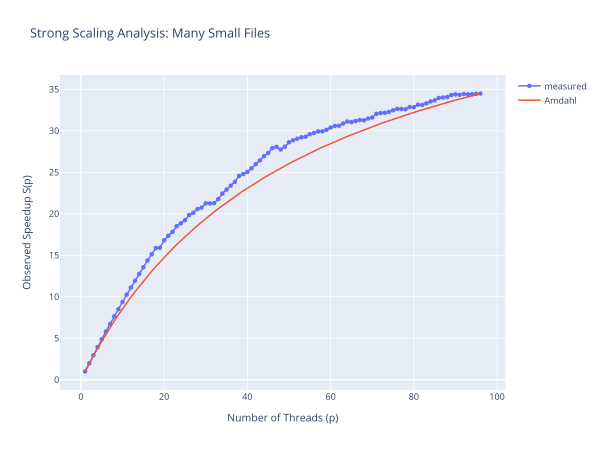
\includegraphics[width=0.7\textwidth]{../results/plots/many_small/speedup_many_small.pdf}
    \caption{Strong scaling analysis for compressing many small files. Measured speedup compared to theoretical Amdahl prediction.}
    \label{fig:many_small}
\end{figure}

\subsection*{One Large File}
We tested compression of a single 512MB file generated using \texttt{dd} from \texttt{/dev/urandom}. Parallelism here is achieved solely by splitting the file into blocks. Figure~\ref{fig:one_large} shows the speedup heatmap varying threads and block size. Maximum speedup (around 23x) is achieved with the maximum number of threads (96) and a block size of approximately 6 MiB. Smaller block sizes (e.g., 1 MiB) perform noticeably worse, likely due to the increased relative overhead of managing metadata and thread synchronization for a very large number of small blocks within a single file context. Larger block sizes (>= 10 MiB) also reduce performance, probably by limiting the available parallelism (fewer blocks than threads) and increasing the chance of load imbalance if some blocks compress much slower than others. The 6 MiB block size seems to strike a good balance for this specific single-file scenario on this architecture.

\begin{figure}[H]
    \centering
    % Updated path relative to report/report_LL.tex
    \includegraphics[width=0.7\textwidth]{../results/plots/one_large/speedup_matrix_one_large.pdf}
    \caption{Heatmap: Speedup vs Threads \& Block Size for one 512 MiB file.}
    \label{fig:one_large}
\end{figure}

\subsection*{Many Large Files}
This scenario, using 10 files ranging from 100 MiB to 250 MiB, allows exploring different nested parallelism strategies. The sequential dispatch approach processes files one after another, parallelizing only the block compression within each file. As indicated in Figure~\ref{fig:many_large_seq}, speedup increases with the number of inner threads, peaking around 18x with 96 threads and favoring small block sizes (1-2 MiB). This method, however, underutilizes resources by foregoing inter-file parallelism. The optimal small block size aligns with maximizing intra-file parallelism when it is the sole source available.

An alternative strategy uses oversubscribed nesting, parallelizing both the outer loop over files and the inner loop over blocks independently. Figure~\ref{fig:many_large_over} plots speedup against the number of outer threads ($p_{outer}$) and block size, assuming the inner loop uses the maximum available threads (96). Peak speedup, approximately 30x, surprisingly occurs when $p_{outer}$ is near the number of files (10) and employs a larger block size of 6-7 MiB. This suggests benefit in assigning primary threads per file, while the preference for larger blocks might stem from reduced synchronization frequency and overhead amortization under the heavy contention caused by extreme oversubscription ($10 \times 96$ potential threads). Although achieving the highest peak speedup here, this method's performance can be sensitive and potentially inefficient due to OS scheduling challenges.

The controlled nesting strategy partitions the total thread budget $P$ using the heuristic $t_{out} = \lceil \sqrt{P} \rceil$ and $t_{in} = \lfloor P / t_{out} \rfloor$ to prevent total active threads from exceeding $P$. Figure~\ref{fig:many_large_ctrl} demonstrates good scalability with the total thread count $P$. Maximum speedup reaches approximately 23x with 96 total threads, favoring small block sizes (1-2 MiB). Preventing oversubscription allows the system to benefit from finer-grained parallelism, akin to the sequential dispatch case but now effectively combined with file-level parallelism. This approach provides robust and predictable scaling, making it generally preferable despite a slightly lower peak performance compared to the oversubscribed method in this specific test.

\begin{figure}[H]
    \centering
    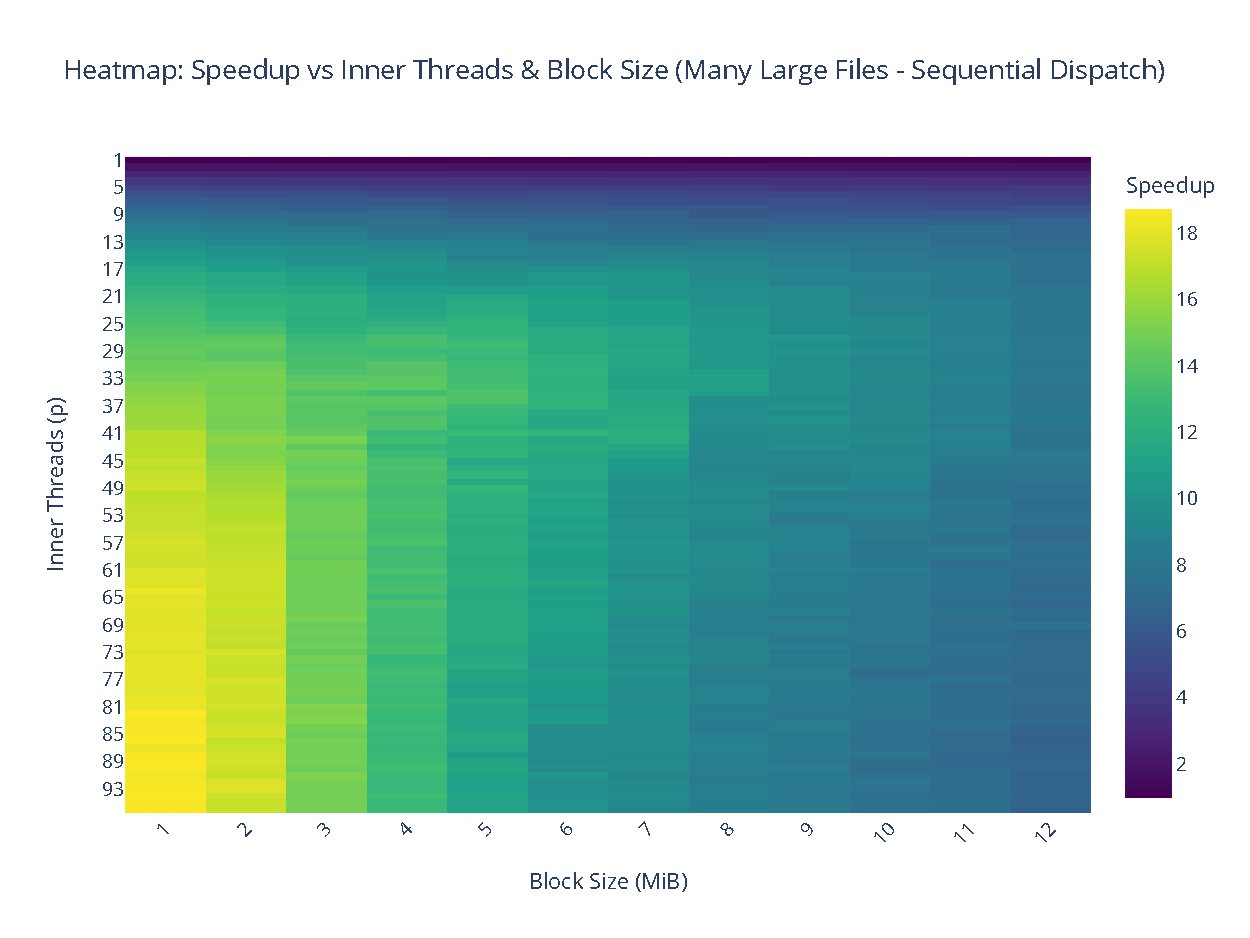
\includegraphics[width=0.7\textwidth]{../results/plots/many_large_sequential/speedup_matrix_many_large_sequential.pdf}
    \caption{Sequential Dispatch: speedup vs inner threads and block size for 10 large files.}
    \label{fig:many_large_seq}
\end{figure}

\begin{figure}[H]
    \centering
    \includegraphics[width=0.7\textwidth]{../results/plots/many_large_parallel/speedup_matrix_many_large_parallel.pdf}
    \caption{Oversubscribed Nesting ($p_{\text{inner}}=96$): speedup vs outer threads and block size.}
    \label{fig:many_large_over}
\end{figure}

\begin{figure}[H]
    \centering
    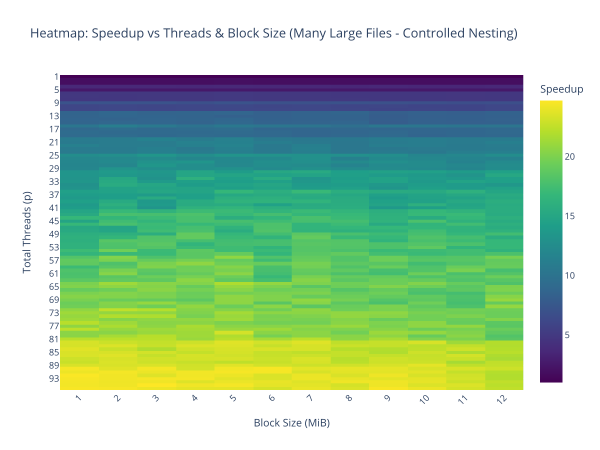
\includegraphics[width=0.7\textwidth]{../results/plots/many_large_parallel_right/speedup_matrix_many_large_right.pdf}
    \caption{Controlled Nesting ($t_{\text{out}}\times t_{\text{in}}\le P$): speedup vs total threads and block size.}
    \label{fig:many_large_ctrl}
\end{figure}

% Regarding the underlying hardware architecture, this Miniz-based compression workload appeared largely insensitive to the NUMA characteristics of the dual-socket test machine, a contrast perhaps to memory-bandwidth or latency-critical applications. Speedup generally scaled well with the total number of available cores up to the machine's capacity, lacking significant performance deviations that would strongly suggest NUMA bottlenecks related to cross-socket data access. This behavior implies the task is predominantly CPU-bound. Factors such as the use of \code{mmap} for efficient I/O and OpenMP's potential for thread affinity likely help localize data access or mask remote access latencies. Consequently, performance seems governed primarily by CPU throughput, thread management overheads (particularly evident under oversubscription), and the trade-offs inherent in block size selection, rather than by challenges related to NUMA memory placement.


\end{document}
